\documentclass[english,a4paper,12pt,oneside]{article}


%\includeonly{lab4}

%Drafting options
%uncomment for double spacing
%\doublespacing

% \usepackage{acronym}
\usepackage{times}
\usepackage{setspace} 
\usepackage{amsmath}    % need for subequations
\usepackage{graphicx}   % need for figures
%\usepackage{picture}
% \usepackage{wrapfig}
\usepackage{graphics}
 \graphicspath{{./}{../data/}}
 \usepackage{epstopdf}
\usepackage{color}
\usepackage{listings}
\lstset{language=C++,
	basicstyle=\ttfamily\footnotesize,
	breaklines=true,
%    basicstyle=\ttfamily,
    keywordstyle=\color{blue}\ttfamily,
    stringstyle=\color{red}\ttfamily,
    commentstyle=\color{green}\ttfamily,
%    morecomment=[l][\color{magenta}]{\#}
}
\usepackage{verbatim}   % useful for program listings
\usepackage{color}      % use if color is used in text
\usepackage{subfigure}  % use for side-by-side figures
\usepackage{varioref}
\usepackage{anysize}
\usepackage{natbib}
\usepackage{fancyhdr}
% \usepackage{units}
\usepackage{longtable}
%\usepackage{bbding}
%\usepackage{aeguill}
\usepackage[hyphens]{url}
\usepackage{hyperref}

\setlength{\parskip}{8pt plus 2pt minus 2pt}
\setlength{\parindent}{0pt}

\marginsize{2cm}{2cm}{2cm}{2cm}
\fancypagestyle{plain}{%
  \fancyhf{}%
  \renewcommand{\headrulewidth}{0pt}%
  \renewcommand{\footrulewidth}{0pt}%
}

\pagestyle{fancy}
%\renewcommand{\sectionmark}[1]{\markright{\thesection.\ #1}}

\renewcommand{\sectionmark}[1]{\markright{#1}{}}
\renewcommand{\subsectionmark}[1]{\markright{#1}{}}
\renewcommand{\subsubsectionmark}[1]{\markright{#1}{}}

%\renewcommand{\quote}[1]{\textit{\begin{quote}#1\end{quote}}}
\newcommand{\bold}[1]{\emph{\textbf{#1}}}

\newcommand{\varentry}[1]{{\guillemotleft}\emph{#1}{\guillemotright}}
\newcommand{\code}[1]{{\tt #1}}

\headheight 10mm


\rhead{22/11/2016}
\chead{}
\lhead{ICP3038 --- Computer Vision}
\rfoot{}
\cfoot{- \thepage  \,\,-}
\lfoot{}

\renewcommand{\headrulewidth}{0.4pt}
\renewcommand{\footrulewidth}{0.4pt} 



\begin{document}
% !TEX root = ./ICP3038_Lab_03.tex

\section*{Laboratory 5: Compute the histogram of the array}

%This is a typical script that you will be working with at each
%laboratory session. To work with these scripts efficiently, follow the
%guidelines below.
%\begin{enumerate}
%  \item The script is not a step-by-step tutorial. It introduces the
%    problem but it is your task to solve it.
%
%  \item If you get stuck, make sure that you read \emph{Help} section
%    at the end of the document.
%
%  \item If you still have problems, ask the lecturer, demonstrator or
%    fellow students for help.
%
%  \item Try to do as much work as possible in the class, where it is
%    easier to get help.
%    
%  \item If you need help when working at home, use the Blackboard
%    discussion board.
%    
%  \item Finish all assignments at least a week before the deadline. If you get
%    stuck, you will still have one week to ask for help.
%\end{enumerate}

The aims of today's lab are:
\begin{itemize}
	\item Finish last week's lab on Sum of Absolute Error (SAE) and normalised cross-correlation (NCC) (it will be useful for the 2\textsuperscript{nd} assignment).
	\item Compute the histogram of the array used last week (also useful for the 2\textsuperscript{nd} assignment). 
\end{itemize}

\section*{Task 0: Finish last week's lab}

Before starting something new, finish the lab from last week. 
%In the lecture, you saw yesterday that it can be extremely complicated to use the IDE to maintain the project files, etc. particularly if students use Windows, Mac, or Linux. 
%There is a ZIP file on Blackboard with 4 (almost) empty C++ source files. There is also a `CMakeLists.txt' file. 
%It is a good practice to organise your source code using directories, etc. Do not compile code in the same directory as your source code. It can get messy... 
%Extract the ZIP file, and set up the compilation environment using \verb+cmake+. 
%In the GUI, the source directory corresponds to the direction in which `CMakeLists.txt' is. 
%The binary directory is where the code will be compiled. Often, we call this directory `bin'. 
%Once the paths are set, press `Configure'. 
%The first time you run the configuration tool, you have to select a generator.
%If you want to use MSVC++ in the lab, make sure to use \emph{Visual Studio 14 2015 Win64}. 
%For Mac OS X, you may want to use the Xcode generator. 
%For Linux, you may choose Makefile. 
%Once the configuration step is over, press `Generate'. 
%The project files are now ready in the `bin' directory. 
%You can compile the code using the preferred IDE.

\section*{Task 1: Compute the histogram}

An histogram is a graphical representation of the intensity distribution in a signal.
It plots the number of samples for each intensity value. 
This definition can be adapted to 2D images:
An histogram is a graphical representation of the pixel intensity distribution in a digital image.
It plots the number of pixel for each intensity value. 

The data is grouped into ranges (such as ``0 to 9'', ``10 to 19'', etc.), and then plotted as bars. 
Each bar represents the number of samples for a range of data. 
Add the method as follows to your class from last week:\\

\begin{lstlisting}
std::vector<unsigned int> getHistogram(unsigned int aNumberOfBins) const;
\end{lstlisting}

As we are using floating-point numbers to store values, we need to define how many bins we want to use. 
In the implementation of the method, you need:
\begin{itemize}
 \item Create an empty \verb+vector+ of $N$ elements (with $N=$~\verb+aNumberOfBins)+ and initialise every element to \verb+0+. All can be done in a single call using the appropriate constructor of \verb+vector+:
 
  \begin{lstlisting}
     // Create an histogram with N bins initialised to 0
     std::vector<unsigned int> p_histogram_data(N, 0);
  \end{lstlisting}

 
 \item Specify the size of a bin. You need to consider the range of values in the array and the number of bins. 
Consider this example ($Y_{noise}$ from last week): The min value is -0.83714 and the max value is 5.3959. So the range is $(5.3959 - -0.83714) = 6.23304$. 
\begin{itemize}
    \item If there is 1 bin, its size is $6.23304 / 1 = 6.23304$.
    \item If there are 2 bins, their size is $6.23304 / 2 = 3.11652$. 
    \begin{itemize}
    	\item The first bin starts at -0.83714 and finishes at $-0.83714 + 3.11652 = 2.27938$.
    	\item The second bin starts at 2.27938 and finishes at $2.27938 + 3.11652 = 5.3959$.
    \end{itemize}
    \item If there are 3 bins, their size is $6.23304 / 3 = 2.07768$. 
    \begin{itemize}
    	\item The first bin starts at -0.83714 and finishes at $-0.83714 + 2.07768 = 1.24054$.
    	\item The second bin starts at 2.27938 and finishes at $1.24054 + 2.07768 = 3.31822$.
    	\item The third bin starts at 2.27938 and finishes at $3.31822 + 2.07768 = 5.3959$.
    \end{itemize}
\end{itemize}
 
 
 \item Count how many values fall into each interval. To do so, for each element of the array, find the index of the bin corresponding to its value. Then increment the bin counter.
\end{itemize}

\section*{Task 2: Save the histogram}

Add the methods as follows to your class:\\

\begin{lstlisting}
void writeHistogram(unsigned int aNumberOfBins, const std::string& aFileName) const;
void writeHistogram(unsigned int aNumberOfBins, const char* aFileName) const;
\end{lstlisting}


Save the histogram as an ASCII file using an \verb+ofstream+. You will need to include \verb+<fstream>+.
\verb+ofstream+ is extremely similar to \verb+cout+. 
The only difference is that the data is stored in a file using \verb+ofstream+. 
To declare a variable of this type and open an output file, just type:
\begin{lstlisting}
std::ofstream output_stream("output.dat"); // Open the file

if (!output_stream.is_open()) // The file is not open
{
	std::string error_message("Cannot open file (output.dat).");
	throw (error_message); // Throw an error
}
output_stream << a1 << " " << b1 << endl;
output_stream << a2 << " " << b2 << endl;
output_stream.close(); // Close the file
\end{lstlisting}
Error checking is important, make sure the file is open before writing in the stream. 

In the case of the histogram, make sure the file contains an header. 
For this purpose, the first line will contain:
\verb+\"Min bin value\" \"Count\"+
Then populate the file. 
Below are examples of output with different number of bins for the file \verb+y_noise.mat+ (file that we used last week).

\subsection*{1 bin}
\begin{center}
\begin{tabular}{cc}
\verb+"+Min bin value\verb+"+ & \verb+"+Count\verb+"+\\
-0.837137 & 401

\end{tabular}
\end{center}

\subsection*{8 bin}
\begin{center}
\begin{tabular}{cc}
\verb+"+Min bin value\verb+"+ & \verb+"+Count\verb+"+\\
-0.837137 &109\\
-0.0580043 &180\\
0.721128 &31\\
1.50026 &28\\
2.27939 &12\\
3.05853 &14\\
3.83766 &14\\
4.61679 &13\\

\end{tabular}
\end{center}

\subsection*{16 bin}
\begin{center}
\begin{tabular}{cc}
\verb+"+Min bin value\verb+"+ & \verb+"+Count\verb+"+\\
-0.837137 & 19\\
-0.447571 & 90\\
-0.0580043 & 124\\
0.331562 & 56\\
0.721128 & 21\\
1.11069 & 10\\
1.50026 & 12\\
1.88983 & 16\\
2.27939 & 9\\
2.66896 & 3\\
3.05853 & 6\\
3.44809 & 8\\
3.83766 & 5\\
4.22722 & 9\\
4.61679 & 7\\
5.00636 & 6\\

\end{tabular}
\end{center}

\section*{Task 3: Plot the histogram}

The resulting file can be loaded in Matlab or Octave to produce a graph that can be included in reports. 
%The same technique applies to your dissertation.

\subsection*{Using Matlab/GNU Octave}

\lstinputlisting[language=matlab,caption=Matlab script to plot the histogram.,label=lst:matlab]{../data/plotHistogram.m}
Listing~\ref{lst:matlab} will use Matlab or GNU Octave\,\footnote{GNU Octave is an opensource project that aims at implementing a free version of Matlab.} to load the file \verb+histogram_y_noise_16bins.txt+, plot the histogram as a bar chart,  and produce two files, an Encapsulated PostScript (EPS) file and a Portable Network Graphics image (PNG) file.
Figure~\ref{fig:matlab} shows the corresponding plots. 

\begin{figure}[!h]
\centering
\subfigure[\label{fig:matlabEPS}EPS file.]{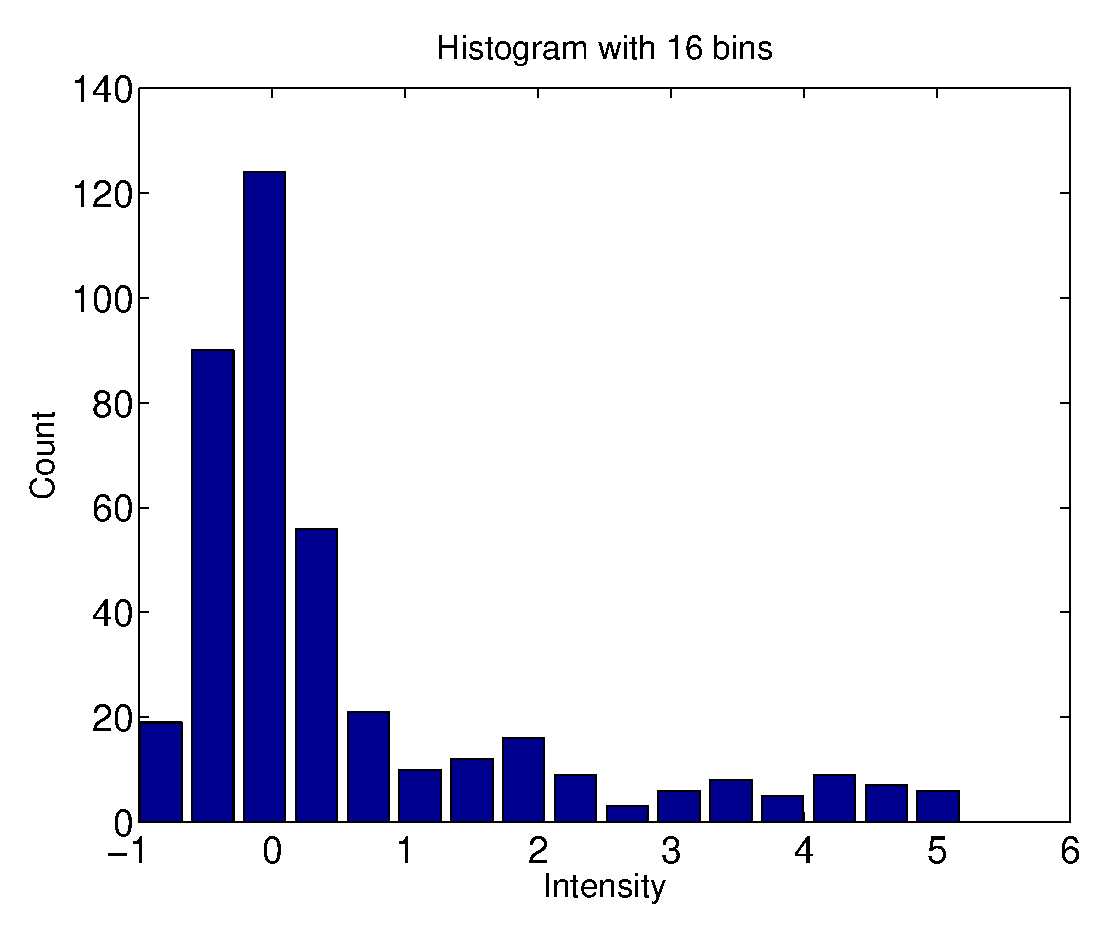
\includegraphics[width=0.45\linewidth]{../data/histogram_matlab.eps}}\hfill
\subfigure[\label{fig:matlabPNG}PNG file.]{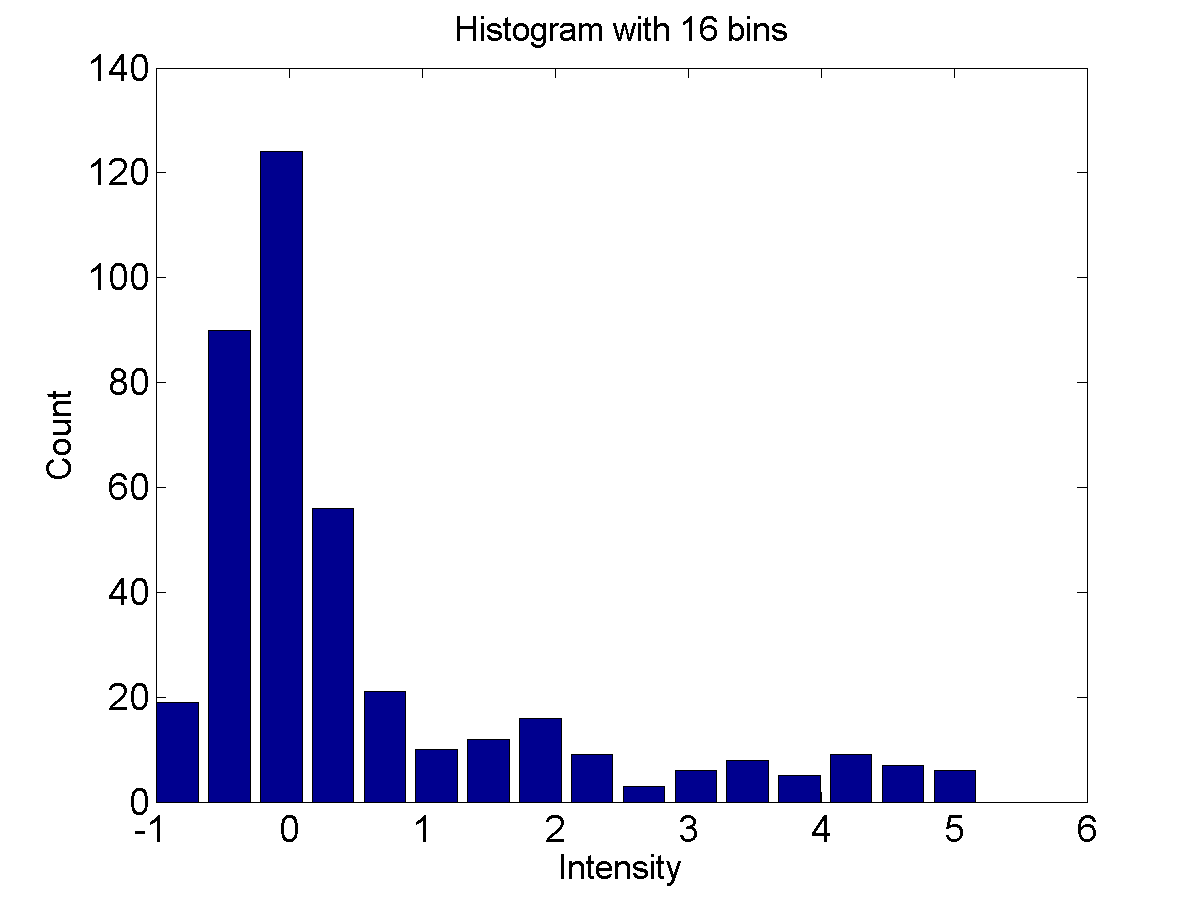
\includegraphics[width=0.45\linewidth]{../data/histogram_matlab.png}}
\caption{\label{fig:matlab}Bar graphs generated using Matlab.}
\end{figure}

\subsection*{Using Gnuplot}

If you do not have Matlab, nor GNU Octave, on your personal, then you can download Gnuplot. 
It is a lighter program dedicated to plot data. 
It can be found at \url{http://www.gnuplot.net/}. 
\lstinputlisting[language=gnuplot,caption=Gnuplot script to plot the histogram.,label=lst:gnuplot]{../data/plotHistogram.plt}

Listing~\ref{lst:gnuplot} will be used with Gnuplot. It will load the file \verb+histogram_y_noise_16bins.txt+, plot the histogram as a bar chart,  and produce another two files (see Figure~\ref{fig:gnuplot}).


\begin{figure}[!h]
\centering
\subfigure[\label{fig:gnuplotEPS}EPS file.]{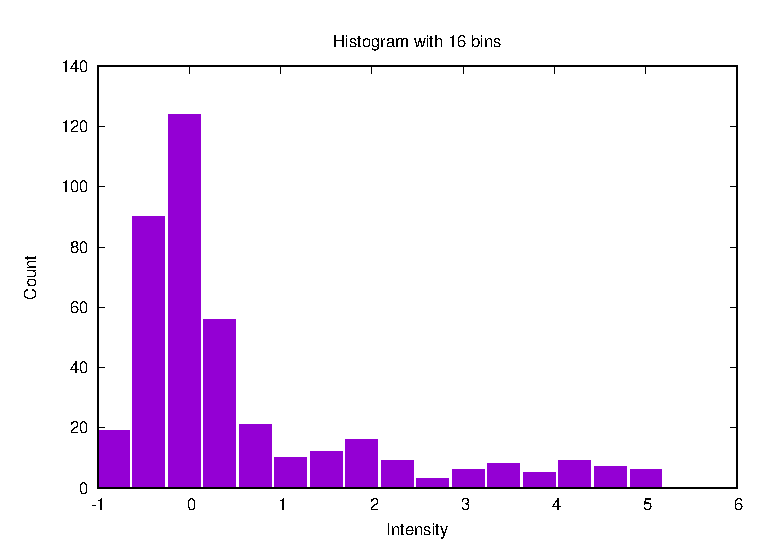
\includegraphics[width=0.45\linewidth]{../data/histogram_gnuplot.eps}}\hfill
\subfigure[\label{fig:gnuplotPNG}PNG file.]{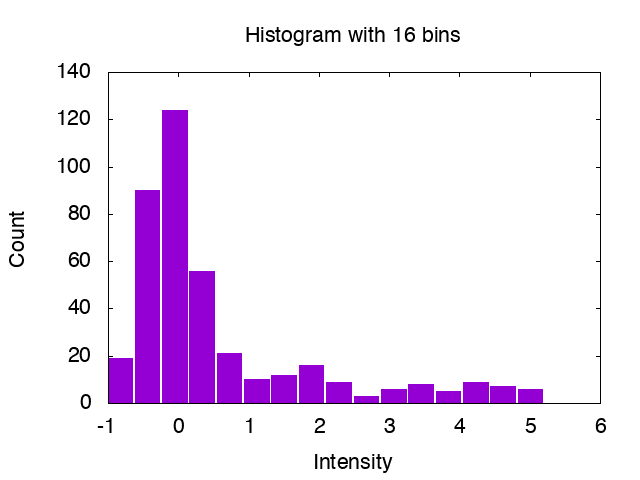
\includegraphics[width=0.45\linewidth]{../data/histogram_gnuplot.png}}
\caption{\label{fig:gnuplot}Bar graphs generated using Gnuplot.}
\end{figure}

\subsection*{Notes on the output files}

The EPS file contains vector graphics and can be zoomed in indefinitely (see Figure~\ref{fig:EPS_zoom}). 
It can be converted as a PDF file (using \verb+epstopdf+ command from the console) and included in reports. 
The PNG file is a bitmap. If you zoom in, it will appear pixelised (see Figure~\ref{fig:PNG_zoom}). 
It is suitable for web pages.

\begin{figure}[!h]
\centering
% trim=l b r t
\subfigure[\label{fig:EPS_zoom}EPS file.]{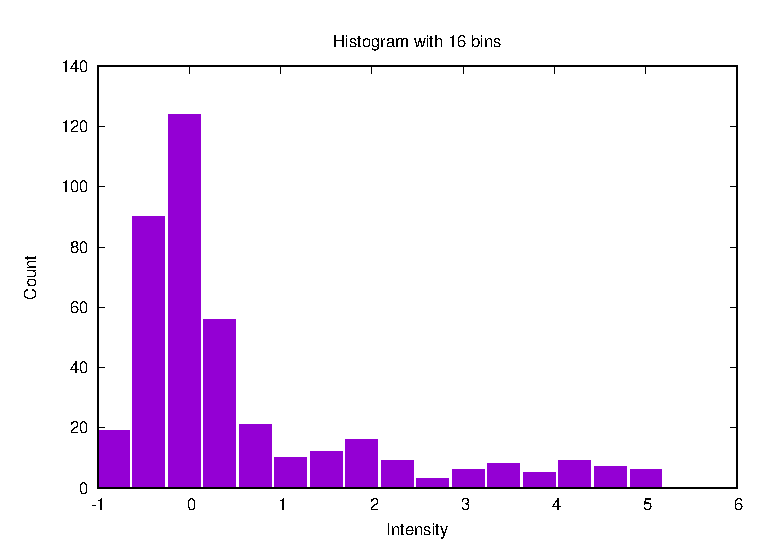
\includegraphics[trim=0mm 5mm 95mm 40mm, clip, width=0.45\linewidth]{../data/histogram_gnuplot.eps}}\hfill
\subfigure[\label{fig:PNG_zoom}PNG file.]{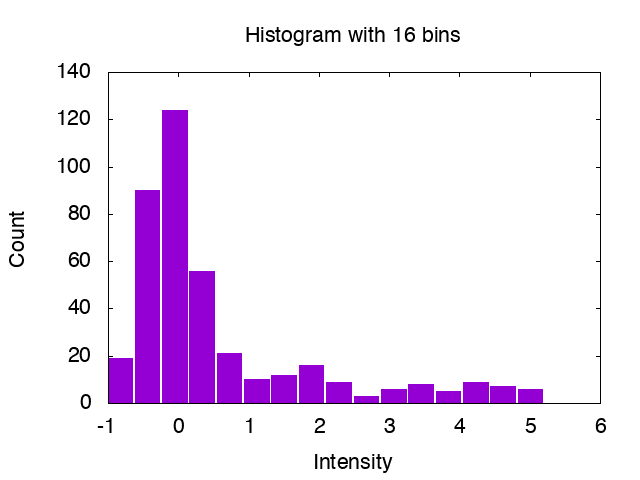
\includegraphics[trim=0mm 10mm 120mm 50mm, clip, width=0.45\linewidth]{../data/histogram_gnuplot.png}}
\caption{\label{fig:zoom}Close up of Figure~\ref{fig:gnuplot}.}
\end{figure}

\section*{Summary}

Today, you saw how to:
\begin{itemize}
\item Compute the histogram of a 1D Array. It is exactly the same for 2D arrays;
\item Plot high-quality graphs.
\end{itemize}
You will re-use similar technique in your next assignment.

%\item $NCC_y_y_quadriple =  99.751$
%\item $NCC_y_y_negative = -99.751$
%\item $NCC_y_y_noise =  96.845$


%
%
%
%
%
%
%For this task, you are given two C++ files:
%\begin{enumerate}
%  \item \verb+include/Utils.h+, a header file with the declarations of some functions.
%  \item \verb+src/TestVector.cpp+, a test program to try the vector class.
%\end{enumerate}
%
%Modify \verb+include/Utils.h+ to convert every function as a template function. 
%To implement every function, you need to write the code directly in the header. 
%In \verb+src/TestVector.cpp+, test every template function with different data types.
%
%
%\section*{Task 3: Create your own template class}
%
%This time, you have to create your own files and modify CMakeLists.txt. 
%We propose to create a template class to handle square matrices, e.g. n-by-n matrices. 
%The class should contain:
%\begin{itemize}
%\item a default constructor, 
%\item a copy constructor, 
%\item a copy operator, 
%\item \verb+operator<<+, 
%\item \verb+operator>>+,
%\item \verb+unsigned int m_size+ (default: 4) the number of rows 
%\item \verb+unsigned int getSize() const+
%\item \verb+void setSize(unsigned int)+
%\item \verb+T& get(unsigned int i, unsigned int j) const+
%\item \verb+void set(unsigned int i, unsigned int j, const T& aValue)+
%\item \verb+void setIdentity()+
%\end{itemize}
%Each method should be tested and validated in a test program. 
%Do not wait until the end to test your code. 
%A good programming strategy is to test a function just after it has been implemented. 
\end{document}
